\documentclass[12pt]{report}

\usepackage[titletoc]{appendix}
\usepackage{datetime}
\usepackage{graphicx}
\usepackage{amsmath}
\usepackage{algorithmicx}
\usepackage{algorithm}
\usepackage[explicit]{titlesec}
\usepackage{tocloft}
\usepackage{amssymb}
\usepackage{longtable}
\usepackage{multirow}
\usepackage[english]{babel}

\usepackage{subcaption}
\usepackage{subfig}

\usepackage{url}

\renewcommand{\familydefault}{\rmdefault}
\renewcommand\cftchapaftersnum{.}
\renewcommand\cftchapdotsep{\cftdotsep}

\setlength{\textheight}{8.63in}
\setlength{\textwidth}{5.9in}
\setlength{\topmargin}{-0.2in}
\setlength{\oddsidemargin}{0.3in}
\setlength{\evensidemargin}{0.3in}
\setlength{\headsep}{0.0in}

\titleformat{\chapter}[block]
  {\Large\filcenter\bfseries}{\MakeUppercase{Chapter \thechapter}\\}{0em}{\MakeUppercase{#1}}
  
\titleformat{\section}[block]
  {\large\bfseries}{\thesection}{0.5em}{#1}
  
\titleformat{\subsection}[block]
  {\normalsize\bfseries}{\thesubsection}{0.5em}{#1}
  

\newcommand{\signature}{\rule{3in}{1.2pt}}
\newcommand{\thesistitle}{Affective Motivational Collaboration Theory}
\newdateformat{monthyear}{\monthname[\THEMONTH] \THEYEAR}

\DeclareMathOperator*{\argmin}{\arg\!\min}
\DeclareMathOperator*{\argmax}{\arg\!\max}

\linespread{1.5}

\begin{document}

\begin{titlepage}
\begin{center}
\large\textbf{\thesistitle}\\[0.5em]

\large\textnormal{by}\\
\large\textnormal{Mahni Shayganfar - mshayganfar@wpi.edu}\\[0.5em]

\large\textnormal{A PhD Dissertation}\\[0.5em]

\large\textnormal{Presented at}\\[0.5em]
\large\textsc{WORCESTER POLYTECHNIC INSTITUTE}\\[0.5em]
\large\textnormal{in partial fulfillment of the requirements for the}\\[0.5em]
\large\textnormal{DOCTOR OF PHILOSOPHY}\\[0.5em]
\large\textnormal{in}\\
\large\textnormal{Computer Science}\\
\large\textnormal{November 2016}\\[0.75em]
\end{center}

\noindent\large\textsc{Approved}\\[0.5em]
\Large\textnormal{\signature}\\
\normalsize\textnormal{Professor Charles Rich, Thesis Advisor}\\[0.5em]
\Large\textnormal{\signature}\\
\normalsize\textnormal{Professor Candace L. Sidner, Thesis Co-Advisor}\\[0.5em]
\Large\textnormal{\signature}\\
\normalsize\textnormal{Professor John E. Laird, Thesis Committee
Member}\\[0.5em] \Large\textnormal{\signature}\\
\normalsize\textnormal{Professor Stacy Marsella, Thesis Committee Member}
\end{titlepage}

\thispagestyle{empty}
\vspace*{\fill}
  \begin{center}
    \textcopyright \hspace{0.5em} Copyright by Mahni Shayganfar 2016

    All Rights Reserved
  \end{center}
\vspace*{\fill}
\newpage

\pagenumbering{roman}

\chapter*{Abstract}
\addcontentsline{toc}{chapter}{Abstract}

Abstract Here!

\pagebreak

\chapter*{Acknowledgments}
\addcontentsline{toc}{chapter}{Acknowledgments}

Acknowledgments Here!

\pagebreak

\tableofcontents
\pagebreak

\listoffigures
\pagebreak

\listoftables
\pagebreak

%\listofalgorithms
%\addcontentsline{toc}{chapter}{List of Algorithms}
%\pagebreak

\pagenumbering{arabic}

\chapter{Introduction}
\label{ch:introduction}

\section{Motivation}

The idea of robots or other intelligent agents living in a human environment has
been a persistent dream from science fiction books to artificial intelligence
and robotic laboratories. Collaborative robots are expected to become an
integral part of humans' environment to accomplish their industrial and
household tasks. In these environments, humans will be involved in robots'
operations and decision-making processes. The involvement of humans influences
the efficiency of robots' interaction and performance, and makes the robots
sensitive to humans' cognitive abilities and behaviors.

A key aspect of the sociability of robots is their ability to collaborate with
humans in the same environment. Collaboration is a coordinated activity in which
the participants work jointly to satisfy a shared goal
\cite{grosz:plans-discourse}. There are many challenges in achieving a
successful collaboration between robots and humans. To meet these challenges, it
is crucial to understand what makes a collaboration not only successful, but
also efficient. Existing computational models of collaboration explain some of
the important concepts underlying collaboration; such as the presence of a
reason for collaborators' commitment, and the necessity of communicating about
mental states in order to maintain progress over the course of a collaboration.
The most prominent collaboration theories are based on plans and intentions
\cite{cohen:teamwork} \cite{grosz:plans-discourse}
\cite{Litman:discourse-commonsense}, and are derived from Bratman's BDI
architecture \cite{bratman:intentions-plans}. Two theories, Joint Intentions
\cite{cohen:teamwork} and SharedPlans
\cite{grosz:planning-acting,grosz:collaboration,grosz:plans-discourse}, have
been used to support teamwork and collaboration between humans and robots or
virtual agents \cite{breazeal:humanoid-robots}
\cite{montreuil:planning-robot-activity} \cite{sidner:enagagement-robot}
\cite{yen:cast}. However, these theories explain only the structure of a
collaboration. For instance, in SharedPlans theory collaborators build a shared
plan containing a collection of beliefs and intentions about the actions in the
plan. Collaborators communicate these beliefs and intentions via utterances
about actions that contribute to the shared plan. This communication leads to
the incremental construction of a shared plan, and ultimately successful
completion of the collaboration. In contrast, in Joint Intentions theory, the
notion of joint intention is viewed as a persistent commitment of the team
members to a shared goal. In this theory, once an agent enters into a joint
commitment with other agents, it should communicate its private beliefs to other
team members.

Although existing collaboration theories explain the important elements of a
collaboration structure, the underlying processes required to dynamically
create, use, and maintain the elements of this structure are largely
unexplained. For instance, a general mechanism has yet to be developed that
allows an agent to effectively integrate the influence of its collaborator's
perceived or anticipated emotions into its own cognitive mechanisms to prevent
shared task failures while maintaining collaborative behavior. Therefore, a
process view of collaboration must include certain key elements. It should
inherently involve social interactions since all collaborations occur between
social agents, and it should essentially constitute a means of modifying the
content of social interaction as the collaboration unfolds. The underlying
processes of emotions possess these two properties, and social functions of
emotions explain some aspects of the underlying processes in collaboration. This
thesis makes the case for emotion-driven processes within collaboration and
demonstrates how it furthers collaboration between humans and robots.

\section{Thesis Statement and Scope}

In this thesis, we develop and validate a framework based on \textit{Affective
Motivational Collaboration Theory} which can improve the effectiveness of
collaboration between agents/robots and humans. This thesis is established based
on the reciprocal influence of collaboration structure and the appraisal
processes in a dyadic collaboration. We focus only on two-participant
collaboration; teamwork collaboration is out of our scope. Furthermore, this
work focuses on a) the influence of emotion-regulated processes on the
collaboration structure, and b) prediction of the observable behaviors of the
other during a collaborative interaction.

We describe the cognitive processes involved in a collaboration in the context
of a cognitive architecture. There are several well-developed cognitive
architectures, e.g., Soar \cite{laird:soar} and ACT-R \cite{anderson:act-r},
each with different approaches to defining the basic cognitive and perceptual
operations. There have also been efforts to integrate affect into these
architectures \cite{dancy:actR-physiology-affect, marinier:behavior-emotion}. In
general, however, these cognitive architectures do not focus on processes to
specifically produce emotion-regulated goal-driven collaborative behaviors. At
the same time, existing collaboration theories, e.g., SharedPlans
\cite{grosz:plans-discourse} theory, focus on describing the structure of a
collaboration in terms of fundamental mental states, e.g., mutual beliefs or
joint intentions. However, they do not describe the associated processes, their
relationships, and influences on each other. \textit{Affective Motivational
Collaboration Theory} deals with some of the major affect-driven processes
having an impact on the collaboration structure. This theory is informed by
research in psychology and artificial intelligence which is reviewed in Chapter
\ref{ch:background}. Our contribution, generally speaking, is to synthesize
prior work on appraisal and collaboration, and motivation to provide a new
theory which describes some of the prominent emotion-regulated goal-driven
phenomena in a dyadic collaboration.

\section{Contributions}

Throughout this work we aim to show how a robot can leverage emotion-driven
processes using appraisal algorithms to improve collaboration with humans. As
such, in this thesis work, we introduce a novel framework, called Affective
Motivational Collaboration (AMC) framework, which allows a robotic agent to
collaborate with a human while incoporating the underlying emotion-driven
processes and the expressed emotion of the human collaborator. Such a framework
is built based on computational models of collaboration and appraisal allowing
for task-driven interaction with robots or other agents. The theoretical
foundation, computational models and algorithms as well as the overall
framework, and the end-to-end evaluation of the framework make the following
contributions:

\begin{enumerate}
  \item \textbf{Introducing \textit{Affective Motivational Collaboration Theory}:}
    
  	(Chapter \ref{ch:amct}) As mentioned earlier, since the theoretical
  	foundation of AMC framework is built on the combination of SharedPlans
  	theory of collaboration \cite{grosz:plans-discourse} and cognitive appraisal
  	theory of emotions \cite{marsella:ema-process-model}
  	\cite{scherer:appraisal-processes}, one of the contributions of our work is
  	to introduce theoretical concepts incorporating key notions of both theories
  	in a dyadic collaboration context. Applying cognitive appraisal theory in the
  	collaboration context is novel. Other models of the appraisal theory have not
  	paid attention to the dynamics of the collaboration.
	
  \item \textbf{Developing new computational models and algorithms for
  \textit{Affective Motivational Collaboration Framework}:}
  
	(Chapter \ref{ch:appraisals}) Another contribution of our work is to create
	computational models and algorithms to compute the value of appraisal variables
	in a dyadic collaboration. We use the collaboration structure to compute
	appraisal variables. Reciprocally, we use the evaluative nature of the
	appraisal to make changes to the collaboration structure as required. We have
	also developed a new algorithm for emotion-driven goal management in the
	context of collaboration. Goal management is one of the important functions of
	emotions during collaboration. Existing models and implementations of emotions
	focus only on how emotions regulate and control internal processes and
	sometimes behaviors. This part of our work shows how appraisal components of
	the self and the human collaborator contributes to goal management as an
	emotion function.
  
  \begin{figure*}
    \centering
    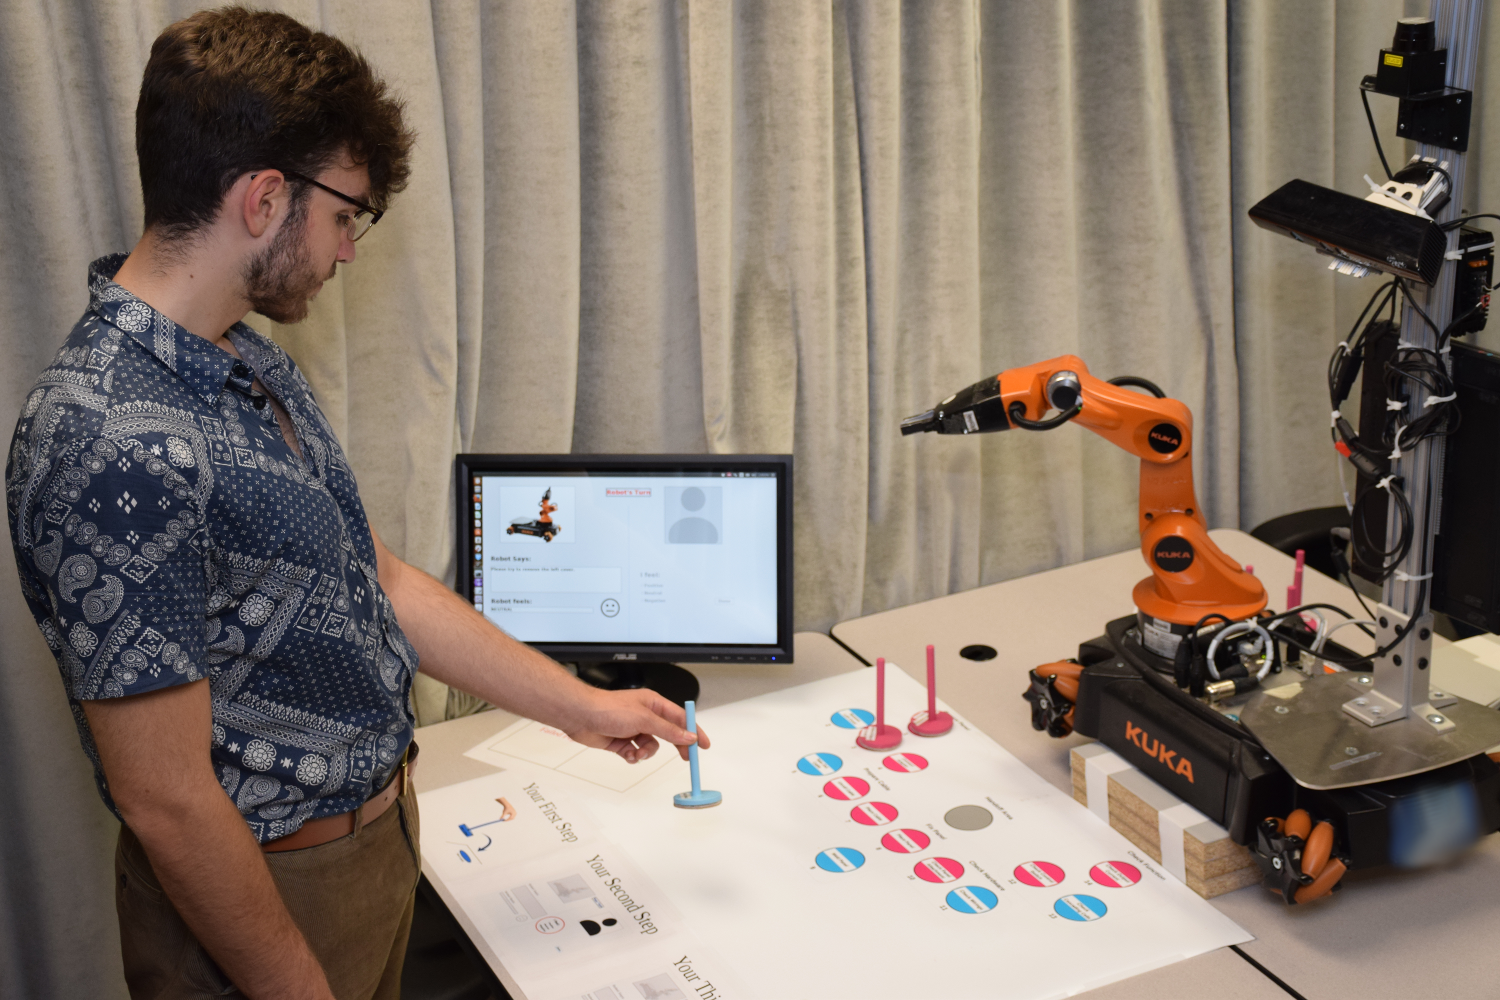
\includegraphics[scale=1.17]{figure/collaborative-robot.png}
    \caption{A robotic arm collaborating with a human to achieve a shared goal
    using \textit{Affective Motivational Collaboration Framework}.}
    \label{fig:collaborative-robot}
  \end{figure*}
  
  \item \textbf{Developing a computational framework based on \textit{Affective
  Motivational Collaboration Theory}:}

  (Chapter \ref{ch:framework}) In order to evaluate our computational models and
  algorithms within an interaction with human collaborators, we have developed
  a computational framework based on our theoretical foundations in
  \textit{Affective Motivational Collaboration Theory}. Our computational
  framework implements the key concepts related to \textit{Affective
  Motivational Collaboration Theory} as well as minimal implementation of other
  processes which are required for validation of the model but are not part of
  this thesis' contributions. The emphasis of the model is on the underlying
  cognitive processes of collaboration and appraisal concepts, rather than the
  Perception and the Action mechanisms.

  \item \textbf{Validating \textit{Affective Motivational Collaboration
  Theory:}}

  (Chapters \ref{ch:appraisals} and \ref{ch:awareness}) We have conducted two
  user studies a) to validate our appraisal algorithms before further
  development of our framework, and b) to investigate the overall functionality
  of our framework within an end-to-end system evaluation with human subjects
  and a robot. The second user study was also conducted to evaluate the benefit
  of using our computational framework in human-robot collaboration. In the
  first user study, we crowd sourced our questionnaires to test our hypothesis
  that humans and our algorithms will provide similar answers to questions
  related to different factors within our appraisal algorithms. In the second
  user study, we investigated the importance of emotional awareness in
  human-robot collaboration, and the overall functionality of the AMC framework
  with the participants in our study environment.
\end{enumerate}

\chapter{Background and Related Work}
\label{ch:background}

\section{Computational Collaboration Theories}

\subsection{Shared-Plans Theory}

\subsection{Joint-Intentions Theory}

\subsection{Hybrid Theories}

\subsection{Similarities and Differences}

\subsection{Applications of Collaboration Theories}

\section{Affective Computing}

\subsection{Affect and Emotions}

\subsection{Functions of Emotions}

\subsection{Motivation and Theory of Mind}

\section{Computational Models of Emotions}

\subsection{Appraisal Theory}

\subsection{Other Computational Models}

\subsection{Similarities and Differences}

\subsection{Applications in Autonomous Agents and Robots}

\chapter{Affective Motivational Collaboration Theory}
\label{ch:amct}

\section{Introduction}

\subsection{Scenario}

\subsection{Example of a Collaborative Interaction}

\section{Design and Architecture}

\subsection{Mechanisms}

\subsection{Functions of Emotions}

\subsection{Mental States}

\subsection{Attributes of Mental States}

\chapter{Appraisal Processes in Collaboration Context}
\label{ch:appraisals}

\section{Introduction}

\section{Appraisal and Collaboration}

\section{Appraisal Algorithms}

\subsection{Relevance}

\subsection{Desirability}

\subsection{Expectedness}

\subsection{Controllability}

\section{Methodology [This chapter will contain the crowdsourding study.]}

\section{Results and Evaluation}

\chapter{Computational Framework}
\label{ch:framework}

\section{System Overview}

\section{Components of the Architecture}

\subsection{Mental States}

\subsection{Collaboration}

\subsection{Appraisal}

\subsection{Coping}

\subsection{Motivation}

\subsection{Theory of Mind}

\subsection{Perception}

\subsection{Action}

\chapter{Improving Human-Robot Collaboration \\ Using Emotional-Awareness}
\label{ch:awareness}

\section{Introduction}

\section{Collaborative Behaviors and Emotional-Awareness}

\subsection{Goal Postponement}

\subsection{Goal Management}

\subsection{Task Delegation}

\section{Methodology}

\section{Results and Evaluation}

\chapter{Conclusion}
\label{ch:conclusion}

\section{Discussion}

\section{Future Work}

\pagebreak

\bibliographystyle{abbrv}
\bibliography{mshayganfar}


\begin{appendices}
\chapter*{Appendix A}
\label{apdx:constraints}
\addcontentsline{toc}{chapter}{A}

\end{appendices}

\end{document}